%%%%%%%%%%%%%%%%%%%%%%%%%%%%%%%%%%%%%%%%%%%%%%%%%%%%%%%%%%%%%%%%%%%%%%%%%%%%%%%%
%2345678901234567890123456789012345678901234567890123456789012345678901234567890
%        1         2         3         4         5         6         7         8

\documentclass[letterpaper, 10 pt, conference]{ieeeconf}  % Comment this line out if you need a4paper

%\documentclass[a4paper, 10pt, conference]{ieeeconf}      % Use this line for a4 paper

\IEEEoverridecommandlockouts                              % This command is only needed if 
                                                          % you want to use the \thanks command

\overrideIEEEmargins                                      % Needed to meet printer requirements.

% See the \addtolength command later in the file to balance the column lengths
% on the last page of the document

%%%%%%%%%%%%%%%%%%%%%%%%%%%%%%%%%%%%%%%%%%%%%%%%
\usepackage[english]{babel}                         
\selectlanguage{english}

\usepackage{amsfonts}
\usepackage{amsmath}
\usepackage{amssymb}

\DeclareMathOperator*{\argmin}{arg\,min}
\DeclareMathOperator*{\argmax}{arg\,max}

\usepackage{graphicx}
\DeclareGraphicsExtensions{.pdf,.eps,.png,.jpg} 
\graphicspath{{./fig/}}
\usepackage{subcaption}

\usepackage{tikz}
\usepackage{tikzscale}
\usepackage{gnuplot-lua-tikz}

\newcommand{\includetexfig}[1]{\input{fig/#1.tex}}

\usetikzlibrary{shapes,fit,positioning}

\tikzstyle{state}=[circle,draw,thick]
\tikzstyle{observation}=[regular polygon,regular polygon sides=4,inner sep=1pt,draw,thick]

\tikzstyle{edata}=[draw,thick,rounded corners,minimum height=.7cm,text width=1.5cm,align=center]
\tikzstyle{data}=[above,text width=1.5cm,align=left]
\tikzstyle{process}=[rectangle,draw,thick,minimum height=.7cm,text width=1.5cm,align=center]
\tikzstyle{io}=[]

\usepackage{booktabs}
%\usepackage[labelfont=bf,width=.8\linewidth,font={small,it}]{caption}
\newcommand{\crefrangeconjunction}{--}
\usepackage[capitalize]{cleveref}
%%%%%%%%%%%%%%%%%%%%%%%%%%%%%%%%%%%%%%%%%%%%%%%%


\title{\LARGE \bf
Visual-Audio Object Recognition Using Hidden Markov Models
}


\author{Weipeng He and Jianwei Zhang$^{1}$% <-this % stops a space
\thanks{*This work was not supported by any organization}% <-this % stops a space
\thanks{$^{1}$W. He and J. Zhang are with TAMS, Department of Informatics, University of Hamburg, Vogt-K\"olln-Str. 30, 22527 Germany. {\tt\small 2he,zhang@informatik.uni-hamburg.de}}%
}

\begin{document}

\maketitle
\thispagestyle{empty}
\pagestyle{empty}

%%%%%%%%%%%%%%%%%%%%%%%%%%%%%%%%%%%%%%%%%%%%%%%%%%%%%%%%%%%%%%%%%%%%%%%%%%%%%%%%
\begin{abstract}
This work aims to implement a system for object recognition given videos of interactions with objects and investigate different modality fusion methods. The system uses the bag-of-words model with SIFT descriptors as the visual feature and the MFCCs as the audio feature. The system classify objects by computing the probabilities with learned hidden Markov models. Two different fusion methods are used in the system: feature fusion and decision fusion. The former method learns a joint probability distribution with one HMM, while the latter method learns two separate distributions for each modality and combine them under the conditional independence assumption. Experiments based on a dataset of 33 different household objects are carried out to evaluate the performance of these two fusion methods as well as unimodal approaches. The result shows that both fusion methods outperform unimodal methods, while these two methods are mostly comparable. 
\end{abstract}

%%%%%%%%%%%%%%%%%%%%%%%%%%%%%%%%%%%%%%%%%%%%%%%%%%%%%%%%%%%%%%%%%%%%%%%%%%%%%%%%
\section{INTRODUCTION}
Humans not only use vision for object recognition, but also perceptions of other modalities, such as auditory, haptic and olfactory perceptions. These extra perceptions provide complementary information. This idea of multimodal object recognition can also be applied to robotic systems.

Traditional object recognition systems, which are exclusively based on visual information, are limited in several ways. They are sensitive to a number of image transformations such as view point change, occlusion and lighting variation. There are also cases where the visual information alone is not sufficient to distinguish an object. For example, a paper cup might have the same appearance as a ceramic cup, and it is difficult to distinguish them only with vision. However, if we strike or touch them, we can get auditory or haptic feedback, from which it is possible to tell the difference.

\section{RELATED WORK}

Nakamura et al.~\cite{nakamura_multimodal_2007} proposed an unsupervised object categorization method for robots based on visual, audio and haptic information. In their experiment, a robot hand was used to grasp and shake the objects. They first extracted scale invariant feature transform (SIFT) descriptors for vision, mel-frequency cepstrum coefficients (MFCCs) for audio and pressure data for haptic information. Then, the bag-of-words models were used to represent all the input information. For categorization, they used a multimodal probabilistic latent semantic analysis (pLSA) model, which is extended from the pLSA model for visual object categorization~\cite{sivic_discovering_2005}.

Sinapov and Stoytchev~\cite{sinapov_object_2011} proposed a behavior-grounded relational learning method for multimodal object recognition. They used an upper-torso humanoid robot to interact with the objects and collect proprioceptive and auditory information. The proprioceptive and audio information were further quantized individually with self-organizing map (SOM) to get sequences of SOM state indices. The similarity between two different sequences was calculated with Needleman-Wunch alignment algorithm. With the similarity, they constructed the relational features, which are the similarities to a known object sets. Consequently, they applied discriminative methods, i.e. support vector machine, k-nearest neighbors and Decision Tree, for learning the object category.

\section{Feature Extraction}
\subsection{Visual Processing Pipeline}
As mentioned in \cref{ch:visual}, the bag-of-words models with SIFT descriptors are powerful at representing the visual features of objects among the same category. And, the applications of bag-of-words models have achieved satisfying performance in visual object category recognition. Therefore, we use the bag-of-words models as the visual feature. The visual processing pipeline is shown in \Cref{fig:vpipe}. 

\begin{figure}[t]
  \centering
  \includegraphics[width=\linewidth]{vpipe.tikz}
  \caption{The visual processing pipeline.}
  \label{fig:vpipe}
\end{figure}

First, the image frames from the raw video are taken at frame rate of 5 frames per second. For each image frame, the keypoints are detected using the DoG keypoint detector. Then, the SIFT descriptors of all the keypoints are computed. All the descriptors are quantized using a codebook of visual descriptors, which is prepared in advance. After that, the number of occurrences of the visual ``words'' are counted and represented as a normalized histogram (i.e. the bag-of-words feature). The codebook used in the experiment contains 20 ``words'', thus the visual feature is a sequence of 20-dimensional vectors.

\subsection{Audio Processing Pipeline}
We choose the MFCCs as the audio feature, because the MFCCs have been commonly used in related fields, such as speech recognition, speaker recognition as well as music information retrieval. The audio processing pipeline is shown in \Cref{fig:apipe}.

\begin{figure}[t]
  \footnotesize
  \centering
  \includegraphics[width=\linewidth]{apipe.tikz}
  \caption{The audio processing pipeline.}
  \label{fig:apipe}
\end{figure}

The audio data are sampled at 8000 Hz. We first use shifting windows with window size of 2048 and shifting size of 1600 to get the audio frames, so that the rate of the audio frames is equal to that of the visual data. Then, we calculate the Mel-frequency cepstrum coefficients (MFCCs) with 32 filter banks. Among all the coefficients, from the second to the 17th are taken, resulting in a 16-dimensional vector. In this way, we get a sequence of MFCCs as the audio feature.

\section{Classification with HMM}
As the system requires a learning model which accounts for time series data, the HMM is a perfect choice in this case, for its effective application in speech recognition and gesture recognition. Besides, the HMM allows us to estimate the probability, which can be used for further inference in modality fusion.

Classification using HMM requires one model to be learned for each class $c$. The model for class $c$ is learned to describe the distribution of all the instances of this class, that is:
\begin{equation}
  \lambda^c = \argmax_{\lambda} \prod_{\mathbf{x} \in D^c} P(\mathbf{x}|\lambda^c)
\end{equation}
in which $D^c$ is the set of data instances the labels of which are $c$. The models are learned with the Baum-Welch algorithm. Then, when given a new instance of observation sequence, we can approximate the likelihood of a class with the learned model by
\begin{equation}
  P(\mathbf{x}|c) = P(\mathbf{x}|\lambda^c) .
\end{equation}

For specific category recognition, which is a multiclass classification problem, the prediction of a new instance is carried out by choosing the class with the maximum likelihood:
\begin{equation}
  \label{eq:classif_s}
  f(\mathbf{x}) = \argmax_{c} P(\mathbf{x}|c) .
\end{equation}

For generic category recognition, the classification is carried out individually for each category. Thus, predicting whether an instance belongs to a certain category is a binary classification problem. The classification is based on comparing the posterior probability to a given threshold $\theta$:
\begin{equation}
  \label{eq:classif_g}
  f(\mathbf{x}) = 
  \left\{ \begin{array}{l l} +1, & \quad P(c=+1|\mathbf{x}) > \theta; \\ -1, & \quad \text{otherwise.}
  \end{array} \right.
\end{equation}

From Bayesian theory, the posterior probability of a class given the observation is
\begin{equation} \label{eq:posterior}
  P(c|\mathbf{x}) = \frac{P(\mathbf{x}|c)P(c)}{\sum_{c \in \{-1,+1\}} P(\mathbf{x}|c)P(c)}
\end{equation}
in which $P(c)$ is the prior probability of the class.

Considering the fact that randomly selecting objects as dataset is not likely to be the same as randomly drawing a sample in a real world, we notice that the prior probability is hard to estimate. However, if we assume that the prior probabilities are equal, we still can make the same decision by varying the threshold. We will later evaluate the performance of a classifier using area under the receiver operating characteristic curve and such evaluation method is not affected by the threshold. Therefore, by assuming equal prior probabilities, \cref{eq:posterior} can be rewrite as 
\begin{equation}
  \label{eq:postsimp}
  P(c|\mathbf{x}) = \frac{P(\mathbf{x}|c)}{\sum_{c \in \{-1,+1\}} P(\mathbf{x}|c)} .
\end{equation}

As seen from \cref{eq:classif_s,eq:classif_g}, the key for both object recognition tasks is to know the likelihood $P(\mathbf{x}|c)$.

\subsection{Model Selection}
An important issue about HMM is selecting the model size and the observation distribution, i.e. the number of states, the number of components per state and the type of covariance matrix. The model choice can have a dramatic impact on the result.

Models with larger number of states and components are more complex. The covariance matrix can be either a full matrix or a diagonal matrix. The diagonal matrix assumes the feature coefficients are not correlated, thus is simpler than full matrix.

\begin{table}[t]
  \caption{Comparison of simple and complex models.}
  \label{tab:model}
  \centering
  \begin{tabular}{p{.42\linewidth}p{.42\linewidth}}
    \toprule
    \multicolumn{1}{c}{\bfseries Simple Models} & \multicolumn{1}{c}{\bfseries Complex Models} \\ \midrule
    Smaller hypothesis space. & Larger hypothesis space. \\
    Easy to learn. & Hard to learn. \\
    Underfitting. & Overfitting. \\
    \bottomrule
  \end{tabular}
\end{table}

In general, simple models have smaller hypothesis space, which means it is it is easy to learn. However, smaller hypothesis space is less likely to contain target distribution, thus problems of underfitting can occur.

On the other hand, complex models have larger hypothesis space, hence can better approximate the target distribution. However, since the Baum-Welch algorithm does not guarantee MLE, complex models are more prone to local optima. Furthermore, it could also result in overfitting if the training set is not large enough. The comparison of simple and complex models are listed in \cref{tab:model}.

Making decision for the model choice should follow the principle of Occam's razor. Depending on different data, the best choice is the simplest model that can fit the data.

\subsection{Implementation Issues}
Several implementation issues are addressed in the following part.

\subsubsection{Underflow and overflow}

When probabilities accumulate through the data sequence, the values can be significantly larger or smaller than $1$. Such values exceed the precision range of machines. To avoid such underflow and overflow, the computation is performed with the logarithmic values of each variable. 

\subsubsection{Insufficient training data}

As previously described in the Baum-Welch algorithm, the reestimation procedure requires a calculation of state probabilities based on a present estimation. Such state probabilities can be zero especially when the training set is insufficient. When a probability of a state is non-zero only with one or a few observations, it is impossible to estimate the covariance matrix. In the system, the values along the diagonal of the covariance matrices are restricted to be above a minimum value, and such approach solves the problem of insufficient training data. 

\subsubsection{Parallelization}

The training process of the HMM parameters can take very long time. The system incorporates parallel computation with OpenMP. The parallelization increases the speed up to 8 times of the original on a computer with an 8-core CPU.

\section{Methods of Multimodal Fusion}
Having discussed how to extract feature vectors and how to make decision based on it, we now move on to the final part of system design: multimodal signal fusion. The way to fuse the visual and audio information is essential to the object recognition system, that good method makes use of both modalities and avoid noises from unreliable signal.

Multimodal fusion methods may be classified according to the level of fusion into feature fusion, decision fusion and hybrid fusion~\cite{atrey_multimodal_2010}. The feature fusion or early fusion is the approach of combining the multimodal features before they are sent as input of a learning model. The decision fusion or late fusion approach, on the other hand, analyzes each modality independently and then combines the individual decisions to a final result. The hybrid fusion is a combination of the two approaches.

The system incorporates two different designs regarding the fusion method: one with feature fusion and the other with decision fusion. Such methods will be presented in the remaining of this section. The performance of the two methods will be further discussed with experimental results in later chapters.

To ground our discussion, consider the problem of classification using HMM with visual and audio features. The observation is a combination of visual and audio features, $\mathbf{x} = (\mathbf{v}, \mathbf{a})$. To make a decision using \cref{eq:classif_s,eq:classif_g}, we need to compute the joint likelihood $P(\mathbf{v},\mathbf{a}|c)$.

\subsection{Feature Fusion}
\begin{figure}[t]
  \footnotesize
  \centering
  \includegraphics[width=\linewidth]{featurefs.tikz}
  \caption[Block diagram of the feature fusion approach.]{Block diagram of the feature fusion approach. Features of different modalities are first combined at the feature fusion module and then the joint probability is computed directly with the HMM which is learned with the combined feature.}
  \label{fig:featuref}
\end{figure}

The feature fusion is a direct approach that the system learns the HMM with the concatenated features. Therefore the joint likelihood can be approximated with 
\begin{equation}
  P(\mathbf{v},\mathbf{a}|c) = P(\mathbf{v},\mathbf{a}|\lambda_{va}^c)
\end{equation}
in which $\lambda_{va}^c$ are the estimated bimodal HMM parameters. A block diagram of such approach is shown in \Cref{fig:featuref}.

The advantage of feature fusion is that it utilizes the correlation between modalities. Theoretically, if the HMM are properly chosen and well trained, the feature fusion approach can yields optimal estimation of the joint likelihood. However, learning both modalities at the same time increases the hypothesis space and also increases the difficulty of estimating the optimal parameters of the HMM. Furthermore, the video and audio features are required to be synchronized in order to get meaningful combined feature.

\subsection{Decision Fusion}
\begin{figure}[t]
  \footnotesize
  \centering
  \includegraphics[width=\linewidth]{decisionfs.tikz}
  \caption[Block diagram of the decision fusion approach.]{Block diagram of the decision fusion approach. Likelihood of different modalities are first computed individually and then combined at the decision level under the conditional independence assumption.}
  \label{fig:decisionf}
\end{figure}

An alternative approach, the decision fusion, is learning separate HMMs and combine the likelihood at decision level. If we assume the features of different modalities are conditionally independent given the class, the joint likelihood can be computed as
\begin{equation}
  P(\mathbf{v},\mathbf{a}|c) = P(\mathbf{v}|c) P(\mathbf{a}|c) = P(\mathbf{v}|\lambda_v^c) P(\mathbf{a}|\lambda_a^c)
\end{equation}
in which $\lambda_{v}^c$ and $\lambda_{a}^c$ are the estimated HMM parameters for visual and audio features, respectively. A block diagram of such approach is shown in \Cref{fig:decisionf}.

Rather than learning a complex HMM model, the decision fusion approach learns two simple models. Therefore it is more likely to get a optimal estimation of the HMM parameters. However, the fusion is based on the assumption of conditional independence, which sometimes does not hold in reality. In this case, the joint likelihood estimation will be biased.

\section{Experiment and Results}
Experiments based on a visual-audio object dataset were carried out to evaluate different object recognition methods. The methods include feature fusion, decision fusion, visual only and audio only approaches. This chapter describes the experiment and the results.

\subsection{Data}
The dataset consists of videos of interactions with 33 different objects. The objects include household objects such as boxes, mugs, bowls and bottles. The materials of the objects range from ceramic to glass, paper, wood, metal and plastic. Some of the objects contain content inside.

The videos were taken from a webcam at a resolution of $640 \times 480$ pixels and frame rate of 10 frames per second. The sound was recorded from the microphone on the webcam at 16000 Hz. When recording, the object was place in the center of the view and take up a dominant part of the image. There was a few objects in the background.

\begin{figure}[t]
  \centering
  \begin{subfigure}[b]{.8\linewidth}
    \centering
    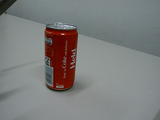
\includegraphics[width=.25\linewidth]{knock0} \hspace{.4cm}
    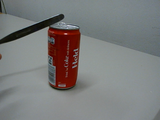
\includegraphics[width=.25\linewidth]{knock1} \hspace{.4cm}
    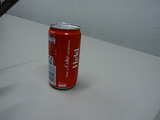
\includegraphics[width=.25\linewidth]{knock2}

    \includegraphics[width=\linewidth]{knock.tikz}
    \caption{Strike}
  \end{subfigure}

  \vspace{20pt}
  \begin{subfigure}[b]{.8\linewidth}
    \centering
    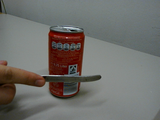
\includegraphics[width=.25\linewidth]{push0} \hspace{.4cm}
    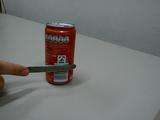
\includegraphics[width=.25\linewidth]{push1} \hspace{.4cm}
    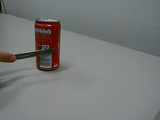
\includegraphics[width=.25\linewidth]{push2}

    \includegraphics[width=\linewidth]{push.tikz}
    \caption{Push}
  \end{subfigure}

  \vspace{20pt}
  \begin{subfigure}[b]{.8\linewidth}
    \centering
    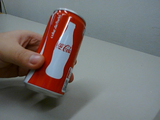
\includegraphics[width=.25\linewidth]{shake0} \hspace{.4cm}
    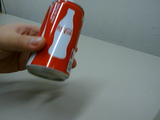
\includegraphics[width=.25\linewidth]{shake1} \hspace{.4cm}
    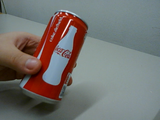
\includegraphics[width=.25\linewidth]{shake2}

    \includegraphics[width=\linewidth]{shake.tikz}
    \caption{Shake}
  \end{subfigure}
  \caption[Interactions with objects.]{Interactions with objects. The images are the video frames during the interaction. The figure below the images is the spectrogram of the sound during the interaction.}
  \label{fig:interaction}
\end{figure}

Three different interactions, including \emph{strike}, \emph{push} and \emph{shake}, were performed by the experimenter. The example videos of the interactions are shown in \Cref{fig:interaction}. Some of the interaction produced sound, while the others did not. Each combination of object and interaction are recorded multiple times from different view points.

Each object is given a set of labels indicating whether this object belongs to a category. Six categories are studied in the experiment, including \emph{mugs}, \emph{bottles}, \emph{plastic objects}, \emph{metal objects}, \emph{fragile objects} and \emph{containers with content}.  
A full list of objects with their categories can be found in \cref{app:dataset}. 

\subsection{Evaluation Criteria}
The performances of the object recognition methods are evaluated with two different criteria for the two different tasks. 
\subsubsection{Evaluation of Specific Object Recognition}
For the specific object recognition task, the accuracy of each method is calculated with 5-fold cross validation. The accuracy (ACC) is the percentage of correctly classified instances, namely 
\[ \text{ACC} =  \frac{\text{\# correctly classified}}{\text{\# total}} . \]
For all methods, the HMM parameters are learned with two states, six mixture components for each state and diagonal covariance matrix.

\subsubsection{Evaluation of Generic Category Recognition}
For the generic category recognition task, we evaluate the classification performance with object-based validation. Each time the video instances of one object is separated from the whole dataset to be the testing data and the rest are used for training. Therefore, all the testing objects are always unseen objects, which are not in the training set. The HMM parameters are learned with various number of states, mixture components and diagonal covariance matrix. For each method, the model with best performance is selected to represent the method.

In the case of generic category recognition, instead of accuracy we used the area under the receiver operating characteristic curve as the criterion. The accuracy does not comprehensively indicate the performance of a binary classifier. It is because there can be cases where more than 90 percents of the instances are negative and a trivial classifier which always predict negative would result in a rather high accuracy.

Since the classification (\cref{eq:classif_g}) is based on a discrimination threshold, it is possible use the receiver operating characteristic (ROC) curve to evaluate the classification result. The ROC curve is generated by plotting the true positive rate (TPR) against the false positive rate (FPR) by shifting the threshold from $0$ to $1$ (\Cref{fig:roc}). The TPR, also known as recall rate or sensitivity, is the percentage of conditionally positive instances being predicted to be positive by the classifier:
\[ \text{TPR} =  \frac{\text{\# true positive}}{\text{\# conditional positive}} . \]
The FPR, also known as fall-out rate, is the percentage of conditionally negative instances being predicted to be positive by the classifier:
\[ \text{FPR} =  \frac{\text{\# false positive}}{\text{\# conditional negative}} . \]

The area under the ROC curve (AUC) can indicate the performance of a binary classifier. An AUC of a classifier is expected to be between $0.5$ and $1.0$, with larger value indicating better performance. The AUC of a random classifier is $0.5$ and that of a perfect classifier is $1.0$.

\section{Results}
\subsection{Specific Object Recognition Results}
The accuracy of each method for the specific object recognition task is shown in \cref{tab:spec}. The performance of both feature fusion and decision fusion methods are better than the visual only and audio only methods. The improvement is about $10\%$. These two fusion methods are only slightly different in performance.

\begin{table}
  \caption{Results of specific object recognition.}
  \label{tab:spec}
  \centering
  \begin{tabular}[h!]{lc}
    \toprule
    \multicolumn{1}{c}{Method} & Accuracy \\ \midrule
    Feature Fusion & \textbf{95.8\%} \\
    Decision Fusion  & 95.7\% \\
    Visual Only & 86.7\% \\
    Audio Only & 83.6\% \\
    \bottomrule
  \end{tabular}
\end{table}

\subsection{Generic Category Recognition Results}
The results of generic category recognition is shown in \cref{tab:cateory} and \Cref{fig:catroc}. For recognition of mugs (\Cref{fig:rocmug}), the decision fusion method has the best performance, followed closely by the visual only method and feature fusion method. For recognition of bottles and plastic objects (\Cref{fig:rocbottle,fig:rocplastic}), both fusion methods are better than the unimodal methods. For recognition of metal objects (\Cref{fig:rocmetal}), the visual only method is the best and the fusion methods are slightly worse. For recognition of fragile objects (\Cref{fig:rocfragile}), the audio only method achieves rather good performance while the visual only method is nearly random. In this case, the performance of both fusion methods are hurt by the visual signals. For recognition of containers with contents (\Cref{fig:rocnonempty}), although all the methods performed poorly, there are improvements with the fusion methods.

On average, both fusion methods are better than the unimodal methods. What is interesting is that the two fusion methods are not only similar in AUC scores, but also their ROC curves appear close to each other. This indicates that they make similar classification results.

\begin{table}
  \caption[Results of generic category recognition.]{Results of generic category recognition. The numbers are the AUC of different methods for the six object categories.}
  \label{tab:cateory}
  \centering
  \begin{tabular}[h]{l*{5}{p{.09\linewidth}}p{.11\linewidth}}
    \toprule
    \multicolumn{1}{c}{Method} & Mugs & Bottles & Plastic Objects & Metal Objects & Fragile Objects & Containers with content \tabularnewline \midrule
    Feature Fusion & 0.750 & \textbf{0.802} & 0.820 & 0.830 & 0.711 & 0.671 \tabularnewline
    Decision Fusion & \textbf{0.771} & 0.798 & \textbf{0.839} & 0.870 & 0.697 & \textbf{0.675} \tabularnewline
    Visual Only & 0.763 & 0.778 & 0.813 & \textbf{0.877} & 0.590 & 0.567 \tabularnewline
    Audio Only & 0.642 & 0.707 & 0.732 & 0.772 & \textbf{0.819} & 0.620 \tabularnewline
    \bottomrule
  \end{tabular}
\end{table}

\begin{figure}[t]
  \footnotesize
  \centering
  \begin{subfigure}[b]{.45\linewidth}
    \includegraphics[width=\linewidth]{mug.tikz}
    \caption{Mugs}
    \label{fig:rocmug}
  \end{subfigure}
  ~
  \begin{subfigure}[b]{.45\linewidth}
    \centering
    \includegraphics[width=\linewidth]{bottle.tikz}
    \caption{Bottles}
    \label{fig:rocbottle}
  \end{subfigure}

  \begin{subfigure}[b]{.45\linewidth}
    \includegraphics[width=\linewidth]{plastic.tikz}
    \caption{Plastic Objects}
    \label{fig:rocplastic}
  \end{subfigure}
  ~
  \begin{subfigure}[b]{.45\linewidth}
    \centering
    \includegraphics[width=\linewidth]{metal.tikz}
    \caption{Metal Objects}
    \label{fig:rocmetal}
  \end{subfigure}

  \begin{subfigure}[b]{.45\linewidth}
    \includegraphics[width=\linewidth]{fragile.tikz}
    \caption{Fragile Objects}
    \label{fig:rocfragile}
  \end{subfigure}
  ~
  \begin{subfigure}[b]{.45\linewidth}
    \centering
    \includegraphics[width=\linewidth]{nonempty.tikz}
    \caption{Containers with content}
    \label{fig:rocnonempty}
  \end{subfigure}
  \caption{ROC curves of generic category recognition results.}
  \label{fig:catroc}
\end{figure}

\section{Conclusion and Future Work}
In this study, we have presented the design and implementation of a visual-audio object recognition system with hidden Markov models. The system has two different modality fusion methods: feature fusion and decision fusion. Experiments were carried out to evaluated the performance of these two methods and unimodal methods.

The results show that, for specific object recognition, both fusion methods increased the accuracy for about 10\%, comparing to unimodal methods. For generic category recognition, both fusion methods increased the performance for most of the categories. Only if one of the input signals is too noisy, the result of the fusion methods will be worse than the result of the good signal. 

The results of the experiments also show that, there is no significant difference between the two fusion methods. One possible explanation for this might be that the visual and audio signals are independent under the condition of being in one category.

It is recommended that further research be undertaken in the following aspects: building a real-time recognition system, increasing the size of dataset and using multimodal signals for feature learning.

The current system cannot perform real-time recognition, for that the extraction of SIFT descriptors requires much computational power and the processing speed is about two frames per second. One possible solution is using SURF descriptors instead of SIFT.

The size of the dataset is critical to the system. With large dataset it is possible to use discriminative methods to learn combination rules. For example, the reliabilities of the modalities can be estimated using a validation set taken from the training set. The reliabilities can be further used for modifying the influence of each signal. To increase the size of the dataset, it is possible to implement robotic systems to automatically collect data or acquire unlabeled data from Internet sources.

Although the performance of a multimodal object recognition system can be improved by finding the optimal combination rule, the upper bound of the performance is decided by the quality of the features. On the hand, thinking of the properties of multimodal signals, for example that the signals appear at the same time contain congruent semantic information, we can actually use the properties as a heuristic for unsupervised learning of good representation. Eventually, the better representation will improve the performance of the recognition system.

%%%%%%%%%%%%%%%%%%%%%%%%%%%%%%%%%%%%%%%%%%%%%%%%%%%%%%%%%%%%%%%%%%%%%%%%%%%%%%%%

\section*{ACKNOWLEDGMENT}

%%%%%%%%%%%%%%%%%%%%%%%%%%%%%%%%%%%%%%%%%%%%%%%%%%%%%%%%%%%%%%%%%%%%%%%%%%%%%%%%

\bibliographystyle{abbrv}
\bibliography{thesis}

\end{document}

